
%(BEGIN_QUESTION)
% Copyright 2011, Tony R. Kuphaldt, released under the Creative Commons Attribution License (v 1.0)
% This means you may do almost anything with this work of mine, so long as you give me proper credit

Calculate the following parameters in this balanced 3-phase electrical power system:

$$\includegraphics[width=15.5cm]{i02328x01.eps}$$

\begin{itemize}
%\item{} $V_{line} =$
%\vskip 10pt
\item{} $I_{line} =$
\vskip 10pt
%\item{} $V_{phase(source)} =$
%\vskip 10pt
\item{} $I_{phase(source)} =$
\vskip 10pt
%\item{} $V_{phase(load)} =$
%\vskip 10pt
%\item{} $I_{phase(load)} =$
\end{itemize}

\underbar{file i02328}
%(END_QUESTION)





%(BEGIN_ANSWER)

\begin{itemize}
\item{} $I_{line} =$ 0.3299 amps
\vskip 10pt
\item{} $I_{phase(source)} =$ 0.1905 amps
\end{itemize}

%(END_ANSWER)





%(BEGIN_NOTES)

{\bf This question is intended for exams only and not worksheets!}.

%(END_NOTES)



